\documentclass[12pt]{article}
\usepackage[spanish]{babel}
\usepackage[utf8]{inputenc}
\usepackage[T1]{fontenc}
\usepackage{geometry}
\usepackage{listings}
\usepackage{mdframed}
\usepackage{amsmath, amssymb, amsfonts, amsthm}
\usepackage{graphicx}
\usepackage{fancyhdr, colortbl}
% paquete para includegraphics
\usepackage{graphicx}
\usepackage{tcolorbox}
\usepackage{tabularx}
\usepackage{array}
\usepackage{colortbl}
\tcbuselibrary{skins}
\usepackage{xcolor}

\pagestyle{fancy}
\fancyhf{} % Limpia los encabezados y pies de página
\fancyhead[L]{Pedro Villar} % Encabezado en la parte izquierda

\definecolor{darkcyan}{HTML}{0091A4}
\definecolor{brightcyan}{HTML}{dcf0f2}

\newmdenv[
topline=false,
rightline=false,
bottomline=false,
leftline=true,
linecolor=darkcyan,
linewidth=3pt,
backgroundcolor=brightcyan,
frametitle=Respuesta
]{rta}

\newcolumntype{Y}{>{\centering\arraybackslash}X}
  \tcbset{tab2/.style={enhanced,fonttitle=\bfseries,fontupper=\normalsize\sffamily,
  colback=white!10!white,colframe=blue!50!black,colbacktitle=blue!40!white,
  coltitle=black,center title}}

\geometry{margin=1.9cm}

\lstdefinestyle{CStyle}{
    language=C,                      % El lenguaje a usar
    basicstyle=\ttfamily\small,      % Tipo de fuente
    keywordstyle=\color{blue},       % Color de palabras clave
    commentstyle=\color{green},      % Color de comentarios
    stringstyle=\color{red},         % Color de strings
    numberstyle=\tiny\color{gray},   % Estilo de los números de línea
    numbers=left,                    % Colocar los números de línea a la izquierda
    stepnumber=1,                    % Numerar todas las líneas
    numbersep=10pt,                  % Separación entre los números de línea y el código
    tabsize=4,                       % Tamaño de las tabulaciones
    showspaces=false,                % No mostrar los espacios como caracteres especiales
    showstringspaces=false,          % No mostrar los espacios en las cadenas de texto
    breaklines=true,                 % Hacer saltos de línea automáticos
    frame=single,                    % Cuadro alrededor del código
}

\lstdefinestyle{BashStyle}{
    language=bash,                    % El lenguaje a usar
    basicstyle=\ttfamily\small,       % Tipo de fuente
    keywordstyle=\color{blue},        % Color de palabras clave (comandos de bash)
    commentstyle=\color{green},       % Color de comentarios
    stringstyle=\color{red},          % Color de cadenas (strings)
    numberstyle=\tiny\color{gray},    % Estilo de los números de línea
    numbers=left,                     % Colocar los números de línea a la izquierda
    stepnumber=1,                     % Numerar todas las líneas
    numbersep=10pt,                   % Separación entre los números de línea y el código
    tabsize=4,                        % Tamaño de las tabulaciones
    showspaces=false,                 % No mostrar espacios especiales
    showstringspaces=false,           % No mostrar espacios en las cadenas de texto
    breaklines=true,                  % Hacer saltos de línea automáticos
    frame=single,                     % Colocar un cuadro alrededor del código
    morekeywords={echo, cd, ls, rm, mkdir}, % Añadir palabras clave de bash
}

\begin{document}

\section*{Práctico 3 - Concurrencia}
\subsection*{Concurrencia}
\noindent \textit{Ejercicio 1.} Dados estos 3 procesos en paralelo:
\begin{figure}[h]
    \centering
    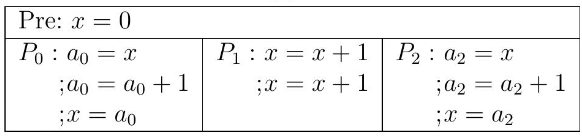
\includegraphics[width=0.5\textwidth]{c1.png}
\end{figure}
\begin{itemize}
    \item[(a)] ¿Qué valores finales puede tomar $x$ ?
    \item[(b)] Muestre para cada uno de los valores un escenario de ejecución que los produzca. Es decir, numere las sentencias y construya la secuencia en base a la numeración.
    \item[(c)] ¿Cuántos escenarios de ejecución hay? * ¿Cuántos para cada valor final de $x$ ?
\end{itemize}

\begin{rta}
    \begin{itemize}
        \item[(a)(b)] Tomando $P_0[i]$ como la línea $i$ del proceso $P_0$, $P_1[i]$ como la línea $i$ del proceso $P_1$ y $P_2[i]$ como la línea $i$ del proceso $P_2$, voy a plantear los distintos escenarios posibles para $x$:
        \begin{itemize}
            \item \textbf{$x$ no  puede ser cero:} en los tres procesos necesariamente incrementan al menos una vez el valor de $x$.
            \item \textbf{$x$ no puede ser mayor a 4:} no hay mas de 4 incrementos en total.
            \item \textbf{$x$ puede ser uno:} en el siguiente escenario $P_0[1]-P_1[1]-P_1[2]-P_2[1]-P_2[2]-P_2[3]-P_0[2]-P_0[3]$.
            \item \textbf{$x$ puede ser dos:} en el siguiente escenario $P_0[1]-P_1[1]-P_1[2]-P_0[2]-P_0[3]-P_2[1]-P_2[2]-P_2[3]$.
            \item \textbf{$x$ puede ser tres:} en el siguiente escenario $P_0[1]-P_2[1]-P_2[2]-P_2[3]-P_0[2]-P_0[3]-P_1[1]-P_1[2]$
            \item \textbf{$x$ puede ser cuatro:} si se ejecutan secuencialmente los procesos:  $P_0[1]-P_0[2]-P_0[3]-P_1[1]-P_1[2]-P_2[1]-P_2[2]-P_2[3]$.
        \end{itemize}
        \item[(c)] Hay $8!$ permutaciones de todas las sentencias, luego hay que sacarles las $(3!2!3!)$ permutaciones de los 3 programas que estan fuera de orden:
        \begin{equation*}
            \frac{8!}{3!2!3!} = 560
        \end{equation*}
    \end{itemize}
\end{rta}

\newpage
\noindent \textit{Ejercicio 2.} Dados estos 2 procesos en paralelo:

\begin{figure}[h]
    \centering
    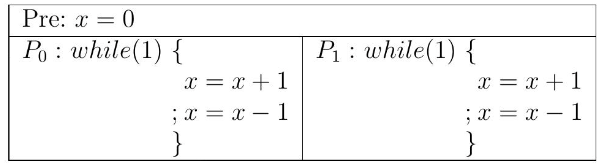
\includegraphics[width=0.5\textwidth]{c2.png}
\end{figure}

\begin{itemize}
    \item[(a)] ¿El multiprograma termina?
    \item[(b)] ¿Qué valores puede tomar $x$?
\end{itemize}

\begin{rta}
    \begin{itemize}
        \item[(a)] Son dos ciclos infinitos, independientemente de que esten ejecutados en paralelo, nunca van a terminar, el planificador va a saltar entre uno y otro.
        \item[(b)] Los programas nos permiten formar cualquier valor en el caso de que las sentencias \textbf{no sean atómicas}, es decir $x$ puede tomar cualquier valor entero. Si son atómicas puede tomar el valor de 0,1,2.
    \end{itemize}
\end{rta}

\noindent \textit{Ejercicio 3.} Considere los procesos:

\begin{figure}[h]
    \centering
    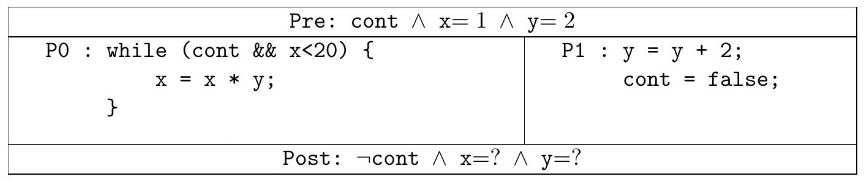
\includegraphics[width=0.7\textwidth]{c3.png}
\end{figure}

\begin{itemize}
    \item[(a)] Calcule los posibles valores finales de x e y.
    \item[(b)] Si en P1 se cambia la instrucción \texttt{y = y + 2}; por \texttt{y = y + 1}; \texttt{y = y + 1}; en dos líneas distintas. ¿Cambia esto los posibles valores finales? Justifique.    
\end{itemize}

\begin{rta}
    \begin{itemize}
        \item[(a)] Y solo va a poder tomar de valor final 2, luego x va a poder tomar los valores : 1,2,4,8,16, 32,64.
        \item[(b)] Al eliminarse la atomicidad de sumarle 2 y dividirla en 2 sumas de 1, estamos permitiendo que la variable $y$ tome mas valores, por lo que ahora el rango de $x$ es distinto: $\{1,2,3,4,6,8,9,12,16,18,24,32,36,48,54,64,72\}$.
    \end{itemize}
\end{rta}

\noindent \textit{Ejercicio 4.} Considere los procesos P0 y P1:

\begin{figure}[h]
    \centering
    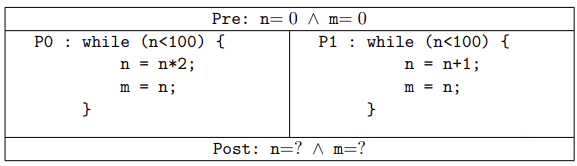
\includegraphics[width=0.5\textwidth]{c4.png}
\end{figure}

\begin{itemize}
    \item[(a)] ¿A cuánto pueden diferir como máximo m y n durante la ejecución?
    \item[(b)] ¿En cuántas iteraciones termina? Indicar mínimo y máximo.
    \item[(c)] ¿Qué valores pueden tomar n y m en la Post? Justifique de manera rigurosa.
\end{itemize}

\begin{rta}
    \begin{itemize}
            \item $n = 2\cdot(m+1)$, esto ocurre en el siguiente escenario: \newline
            \begin{tabular}{|c|c|c|c|}
                \hline
                \rowcolor{cyan!20} % Opcional, para fondo en la fila
                \textbf{Proceso 0} & \textbf{Proceso 1} & \textbf{Valor de n} & \textbf{Valor de m}  \\
                \hline
                - & n = n+1 & n+1 & - \\
                - & m = n & n+1 & n+1 \\
                n = n*2 & - & 2*(m+1) & n+1 \\
                m = n & - & 2*(m+1) & 2*(m+1) \\
                \hline
            \end{tabular} \\
            \item[(b)] \textbf{No hay un máximo definido} y el mínimo es cuando el crecimiento es el máximpo posible, este es cuando n tome los valores 1,2,4,8,16,32,64,128. Es decir, \textbf{el mínimo de iteraciones es 8}.
            \item[(c)] Se pueden tomar todos los valores entre 100 y 200: 
            \begin{enumerate}
                \item \textbf{No puede ser menor que 100: } puesto que si fuese menor a 100, seguiría cumpliendose la guarda dando lugar a que el valor se siga incrementando.
                \item \textbf{No puede ser mayor que 200: } puesto que para que llegue a valer 200, quiere decir que P1 me soló la variable compartida con su valor en 100 y luego P0 me la duplicó, y ya al salir de ahi y concretarse ambos procesos, ninguna de las guardas se va a cumplir.
            \end{enumerate}
    \end{itemize}
\end{rta}

\subsection*{Locks}

\noindent \textit{Ejercicio 5.} La modificación en el punto (b) del Ejercicio 3 introduce cambios en los posibles valores finales, utilice locks para que vuelvan a devolver los mismos valores del punto (a).

\begin{rta}
    \begin{lstlisting}[style=CStyle]
    P0: while (cont && x<20){
        lock(mutex);
        x = x*y;
        unlock(mutex);
    }
    P1: lock(mutex);
        y = y+1;
        y = y+1;
        unlock(mutex);
        cont = false;
    \end{lstlisting}
\end{rta}

\noindent \textit{Ejercicio 6.} Dar una secuencia de ejecución (escenario de ejecución) de las sentencias de dos procesos $P_{0}$ y $P_{1}$ que corren el código de Simple Flag donde ambos entran a la región crítica.

\begin{figure}[h]
    \centering
    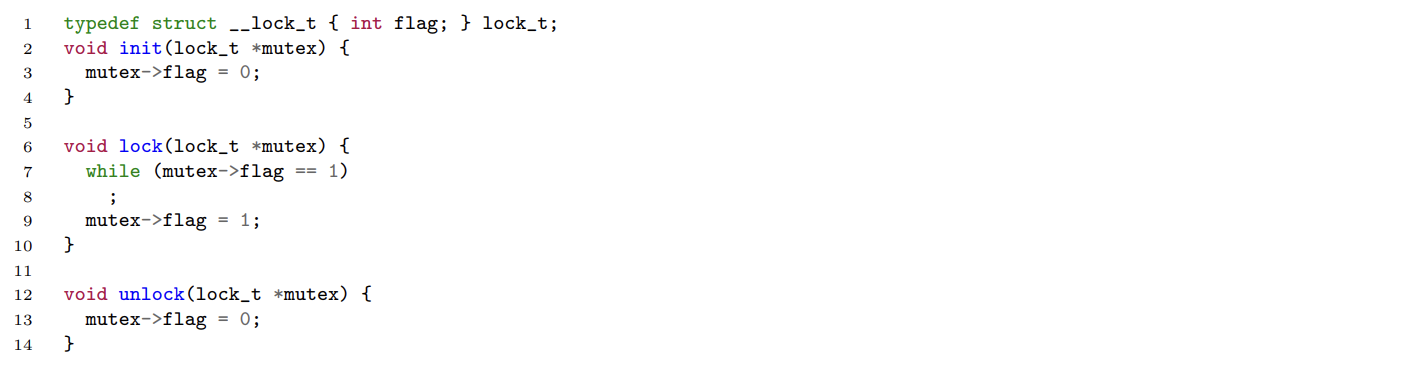
\includegraphics[width=1\textwidth]{c5.png}
\end{figure}

\begin{rta}
    Es una solución que se basa en un flag que indica si un candado esta ocupado o no, acá surge el problema de que dos hilos pueden leer el flag al mismo tiempo y ambos ver que el candado está libre, por lo que ambos intentarán entrar a la sección crítica. Se produce una condición de carrera.
\end{rta}

\noindent \textit{Ejercicio 7.} Hacer una matriz de entradas booleanas para comparar todos los algoritmos de exclusión mútua respecto a características importantes.
\begin{itemize}
    \item Algoritmos: CLI/STI, Simple Flag, Test-And-Set, Dekker, Peterson, Compare-And-Swap, LL-SC, Fetch-And-Add, TS-With-Yield, TS-With-Park.
    \item Características: ¿Correcto?, ¿Justo?, Desempeño, ¿Espera Ocupada?, ¿Soporte HW?, ¿Multicore?, ¿Más de 2 procesos?
\end{itemize}

\begin{table}[htb]
    \refstepcounter{table}\label{tab:mytab}
    \begin{tcolorbox}[tab2,tabularx*={\renewcommand{\arraystretch}{1.5}}{>{\centering\arraybackslash}Y|>{\centering\arraybackslash}Y|>{\centering\arraybackslash}Y|>{\centering\arraybackslash}Y|>{\centering\arraybackslash}Y|>{\centering\arraybackslash}Y},title={Tabla \thetable. Implementaciones del Algoritmo de la Sección Crítica},boxrule=0.8pt]
    \textbf{Solución a la CS} & \textbf{¿Exclusión Mútua?} & \textbf{¿Es justa?} & \textbf{Desempeño} & \textbf{¿MultiCore?} & \textbf{¿Requiere soporte especial del $\mu$P?}  \\\hline\hline
    \textbf{Simple Flag} & NO & NO & Depende de la CS & SÍ & NO \\\hline
    \textbf{Spinlock Test and Set} & SÍ & NO & Depende de la CS y cores & SÍ & SÍ \\\hline
    \textbf{Dekker ('68)} & SÍ & NO & Idem & Dual Core & NO \\\hline 
    \textbf{Peterson ('81)} & SÍ & NO & Idem & Dual Core & NO \\\hline
    \textbf{Test and Set con Yield} & SÍ & NO & Está pensado para una CS grande &  SI & NO \\\hline
    \textbf{Test and Set con Yield, Park, unpark} & SÍ & NO, ya que puede haber deadlock & Está pensado para una CS grande & SI & NO \\\hline
    \end{tcolorbox}
\end{table}

\noindent \textit{Ejercicio 8.} El siguiente programa asegura exlusión mutua en las regiones críticas:

\begin{figure}[h]
    \centering
    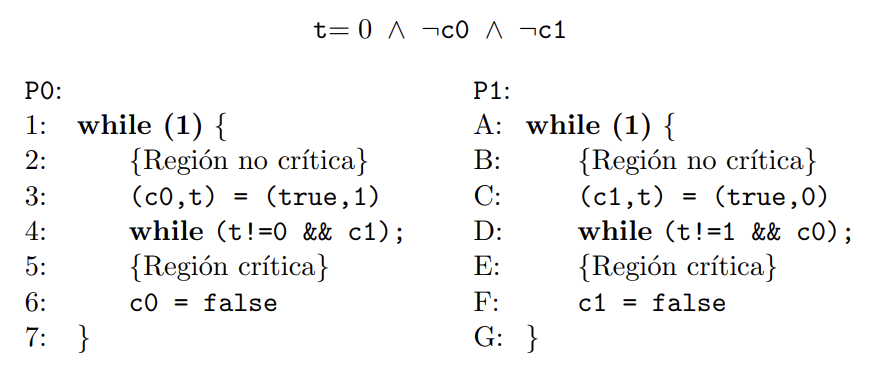
\includegraphics[width=0.5\textwidth]{c6.png}
\end{figure}

Las sentencias 3 y C son asignaciones múltiples que se realizan de manera atómica. Por ejemplo, para el caso de la sentencia 3, las asignaciones $\mathbf{c 0}=$ true y t $=1$ se realizarían en un solo paso de ejecución.

Este protocolo es demasiado exigente en el sentido de que requiere la ejecución de múltiples asignaciones en un sólo paso de ejecución (¡se necesitaría implementar un mecanismo de exclusión mutua en sí mismo para administrar esta atomicidad!). Analice cuál de las 4 posibles realizaciones de este protocolo de exclusión mutua - en el cual las asignaciones ya no son atómicas y por lo tanto hay que darle un orden determinado- es correcta.

\begin{rta}
    Las cuatro posibilidades son las siguientes: \newline
    \textbf{Forma 1: }Esta es la manera correcta de realizar las asignaciones para que haya exclusión mutua en las regiones críticas.
    \begin{lstlisting}[style=CStyle]
    P0: while(true)
        {no CS}
        c0 := true
        t := 1
        while (t != 0 && c1) {}
        {CS}
        c0 := false
    P1: while(true)
        {no CS}
        c1 := true
        t := 0
        while (t != 1 && c0) {}
        {CS}
        c1 := false
    \end{lstlisting}
    \textbf{Forma 2: } Hay un escenario de ejecución en el que ambos quedan en la zona crítica por lo que no se puede asegurar la exclusión mutua. (123ABCDEG457)
    \begin{lstlisting}[style=CStyle]
    P0: while(true)
        {no CS}
        t := 1
        c0 := true
        while (t != 0 && c1) {}
        {CS}
        c0 := false
    P1: while(true)
        {no CS}
        c1 := true
        t := 0
        while (t != 1 && c0) {}
        {CS}
        c1 := false
    \end{lstlisting}
    \textbf{Forma 3: } Hay un escenario de ejecución en el que ambos quedan en la zona crítica por lo que no se puede asegurar la exclusión mutua. (123ABCDEG457)
    \begin{lstlisting}[style=CStyle]
    P0: while(true)
        {no CS}
        t := 1
        c0 := true
        while (t != 0 && c1) {}
        {CS}
        c0 := false
    P1: while(true)
        {no CS}
        t := 0
        c1 := true
        while (t != 1 && c0) {}
        {CS}
        c1 := false
    \end{lstlisting}
    \textbf{Forma 4: } Hay un escenario de ejecución en el que ambos quedan en la zona crítica por lo que no se puede asegurar la exclusión mutua. (ABC123457DEG)
    \begin{lstlisting}[style=CStyle]
    P0: while(true)
        {no CS}
        c0 := true
        t := 1
        while (t != 0 && c1) {}
        {CS}
        c0 := false
    P1: while(true)
        {no CS}
        t := 0
        c1 := true
        while (t != 1 && c0) {}
        {CS}
        c1 := false
    \end{lstlisting}
\end{rta}

\subsection*{Variables de Condición}

\noindent \textit{Ejercicio 9.} Para el siguiente código que intenta implementar productor/consumidor, buscar una falla instanciando dos consumidores y un productor $C_{1}, C_{2}, P_{1}$. Dar una secuencia de líneas que provoca una condición no-deseada.

\begin{figure}[h]
    \centering
    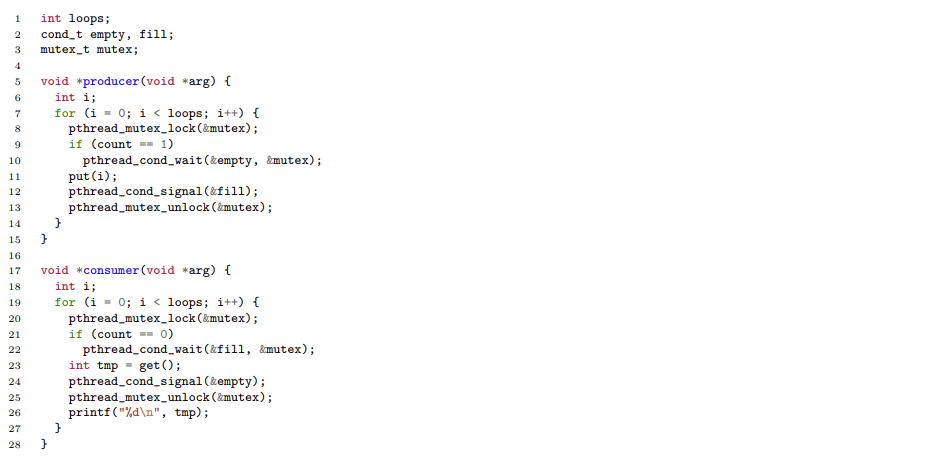
\includegraphics[width=1\textwidth]{c7.png}
\end{figure}

\begin{rta}
    En la columna de consumidor, o productor, se muestran las líneas de ejecución tomando como referencia el código del enunciado, luego se reporta cada acción en la parte de nota. \newline
    \begin{tabular}{|c|c|c|c|c|c|c|}
        \hline
        \rowcolor{cyan!20} % Opcional, para fondo en la fila
        \textbf{C1} & \textbf{Estado} & \textbf{C2}& \textbf{Estado}  & \textbf{P1}& \textbf{Estado}   & \textbf{Nota}  \\
        \hline
        20 & Running          & -  & Ready                & -  & Ready & lock(mutex)         \\
        21 & Running          & -  & Ready                & -  & Ready & condición se cumple \\
        22 & Running          & -  & Ready                & -  & Ready & unlock(mutex)       \\
        -  & Duerme (fill) & 20 & Running              & -  & Ready & lock(mutex)         \\
        -  & Duerme (fill) & 21 & Running              & -  & Ready & condición se cumple \\
        -  & Duerme (fill) & 22 & Running              & -  & Ready & unlock(mutex)       \\
        -  & Duerme (fill) & -  & Duerme (fill)     & 8  & Running & lock(mutex)       \\
        -  & Duerme (fill) & -  & Duerme (fill)     & 9  & Running & condición no se cumple \\
        - & Duerme (fill) & -  & Duerme (fill)      & 11 & Running & cont = 1     \\
        - & Duerme (fill) & -  & Duerme (fill)      & 12 & Running & signal(fill) \\
        - & Duerme (fill) & -  & Duerme (fill)      & 13 & Running & unlock(mutex) \\
        - & Duerme (fill) & -  & Duerme (fill)      & 8  & Running & lock(mutex) \\
        - & Duerme (fill) & -  & Duerme (fill)      & 9  & Running & condición se cumple \\
        - & Duerme (fill) & -  & Duerme (fill)      & 10 & Running & unlock(mutex) \\
        23& Running           & -  & Ready                & -  & Duerme (wait) & cont = 0 \\
        24& Running           & -  & Ready                & -  & Duerme (wait)  & signal(empty) \\
        25& Running           & -  & Ready                & -  & Duerme (wait)  & unlock(mutex) \\
        - & Duerme (fill) & 23  & Running      & 13 & Duerme (wait) & PRE(get) no se cumple \\
        \hline
    \end{tabular}
\end{rta}

\subsection*{Semáforos}

\noindent \textit{Ejercicio 10.} Utilize semáforos para sincronizar los procesos como lo indican los grafos de sincronización. Explicitar los valores iniciales de los semáforos.

\begin{figure}[h]
    \centering
    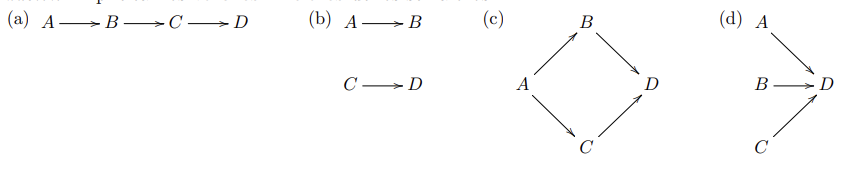
\includegraphics[width=1\textwidth]{c8.png}
\end{figure}

\begin{rta}
    \textbf{Primera sincronización}
    \begin{lstlisting}[style=CStyle]
    sem_init(&s1, 0, 1);
    sem_init(&s2, 0, 0);
    sem_init(&s3, 0, 0);

    A: sem_up(&s1);
    B: sem_down(&s1);
       sem_up(&s2);
    C: sem_down(&s2);
       sem_up(&s3);
    D: sem_down(&s3);
    \end{lstlisting}
    \textbf{Segunda sincronización}
    \begin{lstlisting}[style=CStyle]
    sem_init(&1, 0, 0);
    sem_init(&2, 0, 0);

    A: sem_up(&s1);
    B: sem_down(&s1);
    
    C: sem_up(&s2);
    D: sem_down(&s2);
    \end{lstlisting}
    \textbf{Tercera sincronización}
    \begin{lstlisting}[style=CStyle]
    sem_init(&1, 0, 0);
    A: sem_up(&s1);
    B: sem_up(&s1);
    C: sem_up(&s1);
    D: sem_down(&s1);
    \end{lstlisting}
\end{rta}

\noindent \textit{Ejercicio 11.} Agregar semáforos para sincronizar multiprogramas anteriores.

\begin{itemize}
    \item[(a)] Modifique el programa del Ejercicio 1 agregando semáforos para que el resultado del multiprograma sea determinista (es decir, que no dependa del planificador) y devuelva el mínimo valor posible.
    \item[(b)] Sincronice los procesos del Ejercicio 4 con semáforos de manera que se alternen entre P0 y P1 en cada iteración hasta el final de sus ejecuciones. ¿Qué valores toman n y m al finalizar?    
\end{itemize}

\begin{rta}
    \textbf{Ejercicio 1}
    \begin{lstlisting}[style=CStyle]
    {- PRE: x = 0 -}
    sem_init(&s1, 0, 0);
    sem_init(&s2, 0, 0);
    // Procesos distintos
    P1: a0 := x;
        sem_up(&s1);
        sem_up(&s1);
        x := a0 + 1;
        sem_down(&s2);
        sem_down(&s2);
        x := a0
    P2: sem_down(&s1);
        x :=  x+1
        x := x+1
        sem_up(&s2);
    P3: sem_down(&s1);
        a2 := x
        a2 := a2 + 1
        x  := a2
        sem_up(&s2);
    {- POS: x = 1 -}
    \end{lstlisting}
    \textbf{Ejercicio 4}
    \begin{lstlisting}[style=CStyle]
    {- PRE: n = 0 && m = 0 -}
    sem_init(&s1, 0, 0);
    sem_init(&s2, 0, 1);
    // Procesos distintos
    P0: while(n < 100){
        sem_down(&s1);
        n = n*2;
        m = n;
        sem_up(&s2);
    }
    P1: while(n < 100){
        sem_down(&s2);
        n = n+1;
        m = n;
        sem_up(&s1);
    }
    {- POS: n,m 126,127 -}
    \end{lstlisting}
\end{rta}

\subsection*{Deadlock}
\newpage
\noindent \textit{Ejercicio 12.} Explicar que hace este programa para cada una de las siguientes combinaciones de valores iniciales de los semáforos: $(E, F)=\{(0,0),(0,1),(1,0),(1,1)\}$.

\begin{figure}[h]
    \centering
    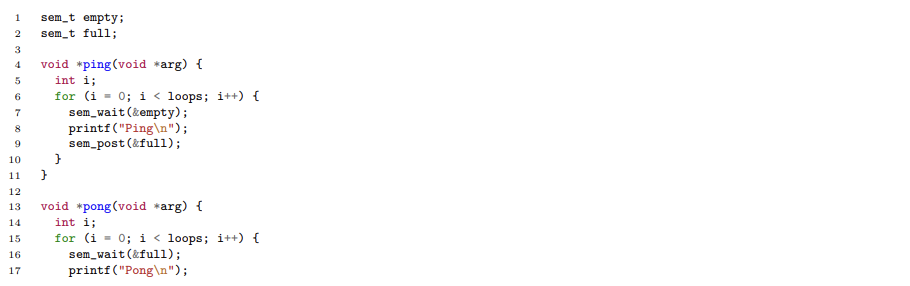
\includegraphics[width=1\textwidth]{c9.png}
\end{figure}
\begin{figure}[h]
    \centering
    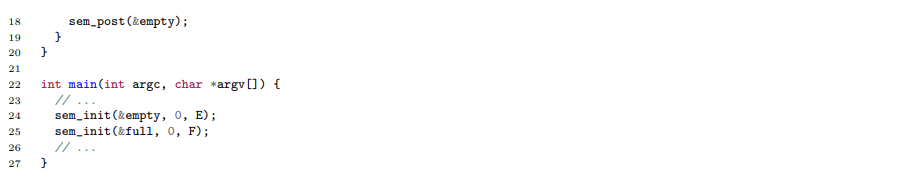
\includegraphics[width=1\textwidth]{c10.png}
\end{figure}

\begin{rta}
    \begin{itemize}
        \item \textbf{Caso (0,0):} Ambos procesos se quedan esperando el semáforo del otro, por lo que se produce un deadlock.
        \item \textbf{Caso (0,1):} Se ejecuta la secuencia pong, ping, pong, ping, ....
        \item \textbf{Caso (1,0):} Se ejecuta la secuencia ping, pong, ping, pong, ....
        \item \textbf{Caso (1,1):} Se ejecutan de manera no determinista, pero siempre se ejecutan de manera alternada.
    \end{itemize}
\end{rta}

\noindent \textit{Ejercicio 13.} ¿Qué primitiva de sincronización implementa el código de abajo con una variable de condición y un mutex?

\begin{figure}[h]
    \centering
    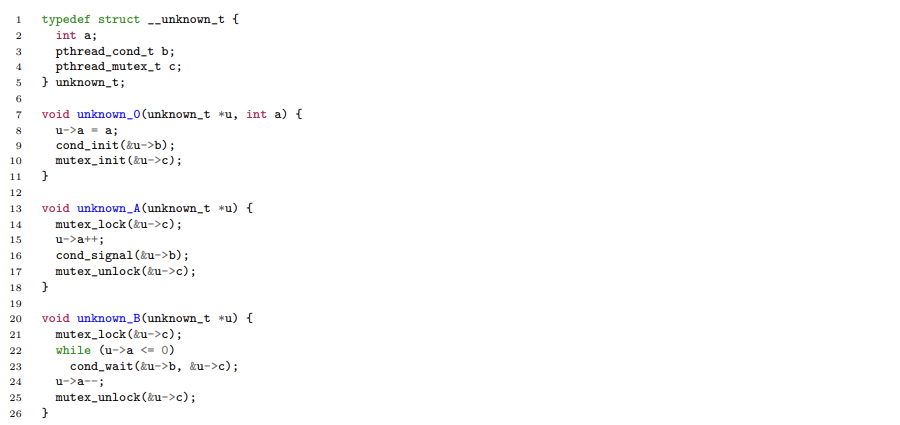
\includegraphics[width=1\textwidth]{c11.png}
\end{figure}

\begin{rta}
    Implementa un semáforo las funciones son:
    \begin{itemize}
        \item \textbf{unknown\_0} es \textbf{sem\_init},
        \item \textbf{unknown\_A} es \textbf{sem\_up},
        \item \textbf{unknown\_B} es \textbf{sem\_down}.
    \end{itemize}
\end{rta}
\newpage
\noindent \textit{Ejercicio 14.} Considere los siguientes tres procesos que se ejecutan concurrentemente:

\begin{figure}[h]
    \centering
    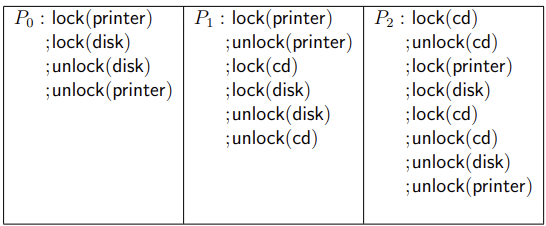
\includegraphics[width=0.6 \textwidth]{c12.png}
\end{figure}

\begin{itemize}
    \item[(a)] Dé la planificación que lleva a un estado de deadlock.
    \item[(b)] Agregue semáforos de manera de evitar que los procesos entren en deadlock. Trate de maximizar la concurrencia.
    \item[(c)] Como solución alternativa, modifique mínimamente el órden de los pedidos y liberaciones para que no haya riesgo de deadlock.
\end{itemize}

\begin{rta}
    \item[(a)] \textbf{Planificación que lleva a un deadlock:} \newline
    \begin{tabular}{|c|c|c|c|}
        \hline
        \rowcolor{cyan!20} % Opcional, para fondo en la fila
        \textbf{Proceso 0} & \textbf{Proceso 1} & \textbf{Proceso 2} & \textbf{Locks tomados}  \\
        \hline\hline
        - & lock(printer) & - & printer \\
        \hline
        - & unlock(printer) & - & - \\   
        \hline
        - & - & lock(cd) & cd \\
        \hline
        - & - & unlock(cd) & - \\
        \hline
        - & - & lock(printer) & printer \\
        \hline
        - & - & lock(disk) & printer,disk \\
        \hline
        - & lock(cd) & - & print,disk,cd \\
        \hline
        - & lock(disk) & - & print,disk,cd (P1 wait disk) \\
        \hline
        - & - & lock(cd) & print,disk,cd (P2,P1 wait cd,disk) \\
        \hline
        lock(printer) & - & - & print,disk,cd (P2,P1,P0 wait cd,disk,printer) \\
        \hline
    \end{tabular} \\
    \textit{Todos se quedan esperando un recurso que otro tiene.} 
    \newpage
    \item[(b)] \textbf{Solución con semáforos:} \newline
    \begin{center}
        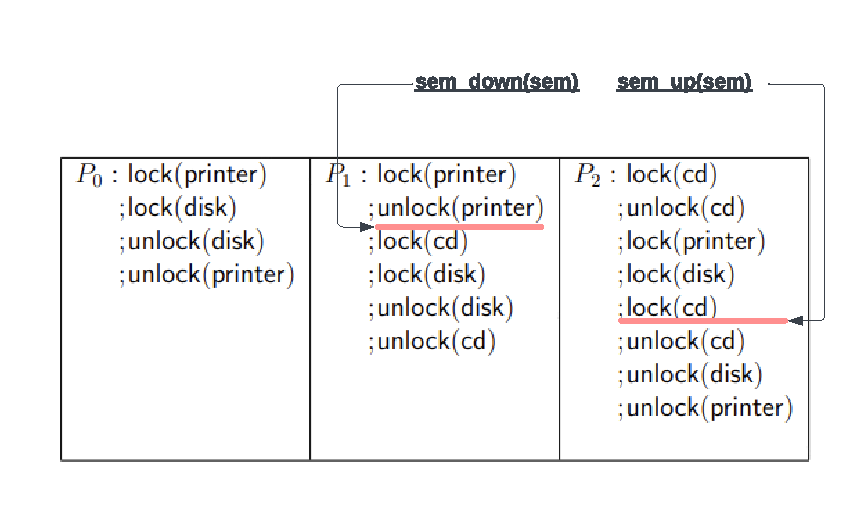
\includegraphics[width=0.7\textwidth]{c13.pdf}
    \end{center}
    \item[(c)] \textbf{Solución alternativa:} \newline
    \begin{center}
        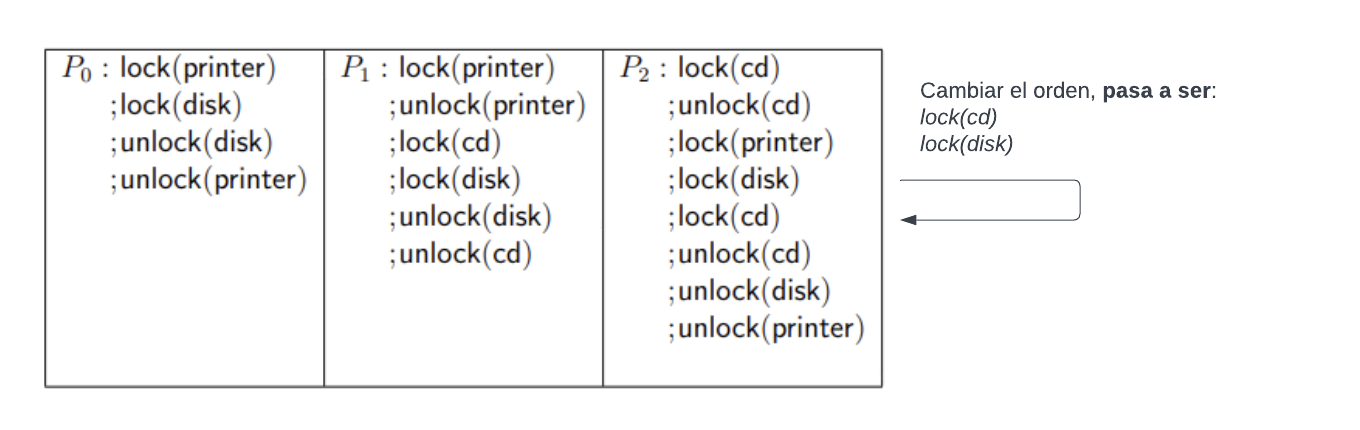
\includegraphics[width=0.8\textwidth]{c14.png}
    \end{center}
\end{rta}


\noindent \textit{Ejercicio 15}. Asuma un sistema operativo donde periódicamente se mata algún proceso al azar. ¿Puede haber deadlock en este contexto?

\begin{rta}
    El deadlock es simplemente un ciclo de espera infinita entre locks, este enfoque no me asegura que no se caiga en ese ciclo, por lo que es probable que se reduzca la probabilida de que ocurra, pero no se elimina.
\end{rta}



\end{document}
